\chapter{Methodology}\label{ch:method}

\section{Dataset curation, preprocessing, and partitioning}
Our experiments use a complete CSV mirror of the AG News titles and descriptions \citep{agmirror,zhang2015} matching the standard \texttt{torchtext} benchmark splits of 120,000 training and 7,600 test articles \citep{torchtext}. Figure~\ref{fig:data-partitions} summarizes how the raw corpus is filtered and partitioned into disjoint subsets for training, validation selection, separate confirmation, and final testing.

\begin{figure}[!b]
\centering
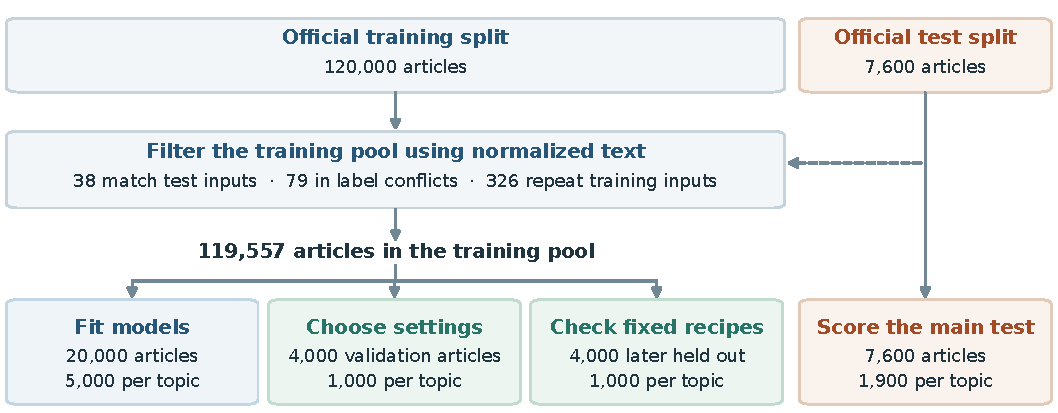
\includegraphics[width=.94\linewidth]{figures/data_partitions.pdf}
\caption[Data filtering and partitions]{Filtering and stratified partitioning of the AG News dataset. Training articles whose normalized text matches an official test article are removed before drawing the disjoint training, validation, and separate confirmation partitions.}
\label{fig:data-partitions}
\end{figure}

During ingestion, every article receives a permanent identifier (\texttt{source\_id}, combining its source split name and zero-based row index), while the four topic labels (\emph{World}, \emph{Sports}, \emph{Business}, and \emph{Sci/Tech}) map to integer class indices $0, 1, 2, 3$. Preserving \texttt{source\_id} across all preprocessing and corruption stages allows clean and corrupted predictions on the exact same article to be paired directly; only the title and description serve as model input.

All models share an identical text normalization pipeline: concatenate title and description separated by a space, convert characters to lowercase, extract contiguous ASCII letter runs via \artifact{[a-z]+}, truncate to at most 128 words, and rejoin tokens with single spaces. Under this rule, hyphenated compounds split into separate words, while digits, punctuation, and currency symbols are discarded. We omit stemming, lemmatization, and stopword removal so both the baseline and the convolutional networks observe natural word order and morphology, and concatenating the fields lets bigrams and convolutional windows bridge the boundary between headline and lead sentence.

To prevent data leakage and label noise before splitting, a deduplication filter checks normalized strings truncated to 128 words across the 120,000-article training pool. It removes 38 training articles that match an official test article exactly, 79 records from duplicate groups with conflicting labels, and 326 redundant copies of repeated training texts (keeping first occurrences), although near-duplicates covering the same news event can remain. The official test split of 7,600 articles (1,900 per class) is kept completely unaltered for benchmark comparability, even though one normalized string appears twice within it.

From the 119,557 surviving training articles, our splitter shuffles each class using seed 2026 and extracts disjoint class-balanced partitions: 20,000 training articles (5,000 per topic) and 4,000 validation articles (1,000 per topic), reused across all main model fits. A separate confirmation sample of 4,000 articles (1,000 per topic) is drawn from the unused filtered pool, excluding records touched in preliminary sanity checks, to test frozen seed-42 recipes on unseen data; a post-split audit verified zero overlap in \texttt{source\_id} or normalized text across the training, validation, confirmation, and official test splits.

Truncating inputs to 128 words sets the fixed padded width for the neural models while ensuring that the baseline scores the exact same document span; only 18 of the 20,000 training articles and five of the 7,600 official test articles exceed 128 words. Stripping non-alphabetic characters, however, removes surface cues whose prevalence differs by category (Figure~\ref{fig:normalization-cues}): currency symbols appear in 17.0\% of raw Business training articles versus at most 6.0\% in any other topic, while numeric digits range from 47.4\% in World to 70.0\% in Sports. Isolating the downstream accuracy effect of retaining digits or currency symbols would require a dedicated preprocessing ablation.

\begin{figure}[!htbp]
\centering
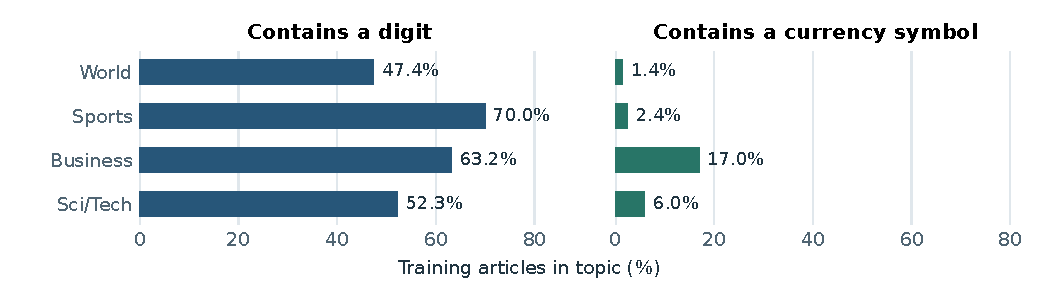
\includegraphics[width=.92\linewidth]{figures/normalization_cues.pdf}
\caption[Raw cues removed by normalization]{Percentage of the 20,000 selected training articles (5,000 per topic) containing numeric digits or currency symbols prior to alphabetic normalization.}
\label{fig:normalization-cues}
\end{figure}

\section{Controlled spelling corruption and training arms}\label{sec:noise}
We model typographical noise through deterministic transpositions of unequal adjacent interior letters. A normalized word is \emph{eligible} for corruption if it has length at least four and contains at least one unequal adjacent pair of interior characters (excluding its first and last letters); words of three or fewer letters (such as \texttt{the} or \texttt{oil}) and words with uniform interiors (such as \texttt{seen}) remain unchanged.

For each article, the corruption routine initializes an independent pseudorandom generator seeded jointly by the global corruption seed and the article's \texttt{source\_id}, guaranteeing identical edits regardless of batching or corpus order. Scanning eligible words from left to right, the generator draws both $u \in [0, 1)$ and a uniformly chosen unequal interior pair for every eligible word before checking whether $u < p$ (Listing~\ref{lst:swap-word}). Drawing both random values prior to the threshold check yields strictly nested corruptions across swap targets $p$: every word swapped at $p = 5\%$ remains swapped in the exact same way at $p = 10\%$ and $p = 20\%$, alongside newly triggered edits.

\begin{lstlisting}[language=Python,keywordstyle=\color{darkgreen},caption={[Core logic for swapping letters in one word]Core logic for swapping letters in one word. The counters are omitted.},label={lst:swap-word},float=htbp]
def swap_word(word, probability, rng):
    candidates = [i for i in range(1, len(word) - 2)
                  if word[i] != word[i + 1]]
    if not candidates:
        return word
    draw, index = rng.random(), rng.choice(candidates)
    if draw >= probability:
        return word
    return word[:index] + word[index + 1] + word[index] + word[index + 2:]
\end{lstlisting}

Validation selection evaluates models at $p \in \{0\%, 10\%\}$, the main official test sweep evaluates $p \in \{0\%, 5\%, 10\%, 20\%\}$ (using corruption seed 41001), the confirmation check evaluates $p \in \{0\%, 10\%\}$, and follow-up sensitivity checks evaluate two extra independent test draws at $p = 20\%$ (seeds 41002 and 41003). Across the 7,600 official test articles (289,990 total words, of which 187,152 are eligible; Figure~\ref{fig:swap-exposure}), $p = 20\%$ transposes 20.03\% of eligible words (12.93\% of all test words, or 37,494 words) and modifies at least one word in 99.1\% of test articles (7,533 of 7,600), because a typical news item contains roughly two dozen eligible words.

\begin{figure}[!htbp]
\centering
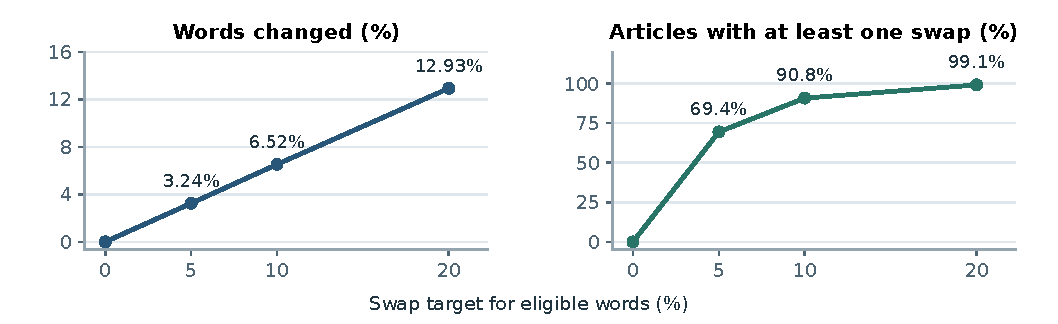
\includegraphics[width=.92\linewidth]{figures/swap_exposure.pdf}
\caption[Realized exposure to spelling swaps]{Realized corruption exposure across the 7,600 official test articles as a function of the swap target for eligible words $p$. Left: percentage of all test tokens modified. Right: percentage of test articles containing at least one modified word.}
\label{fig:swap-exposure}
\end{figure}

To test whether training exposure to spelling swaps improves resilience, we fit every architecture under two parallel training arms:

\paragraph{Clean training arm.}
All 20,000 normalized training articles are presented in their uncorrupted form.

\paragraph{Augmented training arm.}
Within each fitting seed, we sample 50\% of the training articles per topic (2,500 per class, 10,000 total) without replacement, corrupt them at $p = 10\%$, and substitute them in place, keeping corpus size fixed at 20,000 articles (5,000 per class).

In the augmented arm, distinct random streams derived from the fitting seed select the 10,000 articles and apply word swaps. Seed 42 modifies 9,082 of the 10,000 selected articles and 24,791 of the 766,601 training tokens (3.23\%); seeds 43 and 44 modify 24,803 and 24,728 tokens, respectively. Built once per fitting seed prior to vocabulary construction and held static across all models and epochs, in-place replacement alters fitted vocabularies and document frequencies while reducing exposure to clean canonical spellings.

\section{Baseline and neural architectures}\label{sec:models}
All three primary pipelines accept the same normalized article strings and output four class logits (Figure~\ref{fig:model-flow}).

\begin{figure}[!htbp]\centering
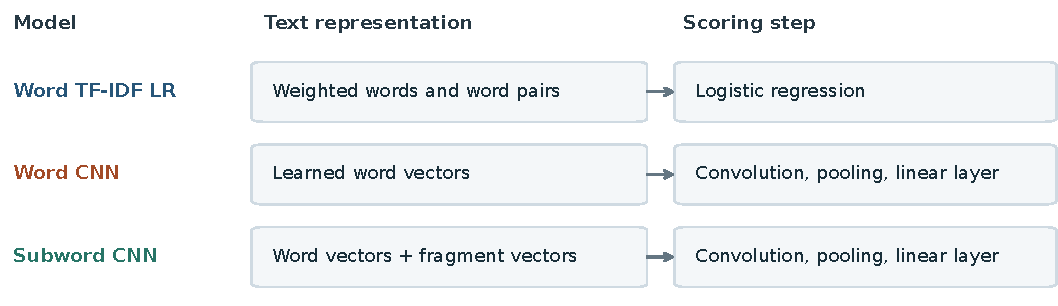
\includegraphics[width=.92\linewidth]{figures/core_prediction_flow.pdf}
\caption[From normalized article to topic scores]{Processing pipelines from normalized text to four topic scores. Subword CNN enriches token representations with hashed character-fragment vectors before applying the same convolutional, pooling, and linear stages as Word CNN.}\label{fig:model-flow}
\end{figure}

\subsection{Word TF-IDF Logistic Regression baseline}
Splitting normalized strings on single spaces guarantees exact token parity with the neural models. Fitted exclusively on the active training arm, \texttt{TfidfVectorizer} extracts word unigrams and adjacent word bigrams with $\mathrm{min\_df} = 2$ (filtering out hapax legomena, including single training typos in the augmented arm), caps the vocabulary at the top 50,000 terms by corpus frequency, and applies the sublinear TF-IDF weighting and $L_2$ row normalization defined in Chapter~\ref{ch:background}.

The resulting 20,000 $\times$ 50,000 training matrix is stored in compressed sparse row format, and validation and test splits are transformed using the frozen training vocabulary and document frequencies so unseen swapped n-grams drop out. Multinomial logistic regression optimizes four 50,000-dimensional weight vectors and four scalar intercepts (200,004 parameters in total) via L-BFGS for up to 1,000 iterations with an $L_2$ penalty controlled by inverse regularization strength $C$. Evaluating $C \in \{0.5, 2.0, 8.0\}$ on the validation objective $J(f)$ selects $C = 2.0$ under clean training and $C = 8.0$ across all three augmented training seeds.

\subsection{Word CNN}
Word CNN builds its lookup table from the active training arm by ranking tokens by descending frequency (breaking ties alphabetically), assigning indices $2, \dots, 29{,}999$ to the top 29,998 words, index 0 to right-padding, and index 1 to the shared unknown token (\texttt{<unk>}), yielding a 30,000-row vocabulary. Validation and test tokens outside those 29,998 words map to index 1, although recurring misspellings can enter the vocabulary: in the original 20\% test draw, 60.9\% of swapped tokens appeared in the vocabulary fitted on augmented text with seed 42.

For a batch of $B$ articles, the encoder outputs a right-padded $B \times 128$ integer matrix alongside true unpadded word counts $\ell \in \{1, \dots, 128\}$. Lookup in the 30,000 $\times$ 96 embedding table produces a $B \times 128 \times 96$ tensor; trainable rows (including \texttt{<unk>}) are initialized from $\mathcal{N}(0, 1)$, whereas padding row 0 is initialized to zero and kept frozen.

Transposing the tensor to $B \times 96 \times 128$ feeds three parallel stride-1 1D convolutional layers (64 filters each at kernel widths $k \in \{3, 4, 5\}$) followed by biased $\operatorname{ReLU}$ activations, yielding $128 - k + 1$ window activations per filter. To prevent right-padding from inflating outputs on shorter documents, our pooling stage applies an explicit length mask: for an article of $\ell$ true words, only the first $\max(1, \ell - k + 1)$ windows are retained (keeping the first window when $\ell < k$), while trailing padded positions are masked to $-\infty$ prior to taking the maximum over time. Concatenating the 64 maximum activations from each width produces a 192-dimensional vector; dropout ($p_{\mathrm{drop}} = 0.5$ during training, disabled at evaluation) precedes a linear head mapping the 192 features to four topic logits (Figure~\ref{fig:word-cnn-forward}).

\begin{figure}[!htbp]\centering
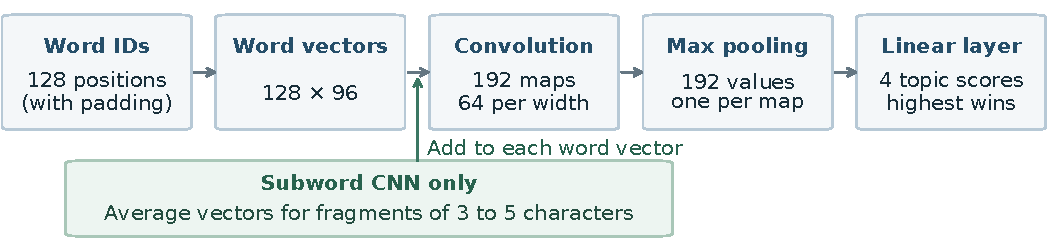
\includegraphics[width=.92\linewidth]{figures/word_cnn_forward.pdf}
\caption[CNN input and output shapes]{Tensor dimensions during the forward pass for a single article in Word CNN and Subword CNN. Subword CNN adds the mean of hashed character-fragment vectors to each word embedding prior to identical convolution, masked max pooling, dropout, and linear classification stages.}\label{fig:word-cnn-forward}
\end{figure}

\subsection{Subword CNN}
Subword CNN retains Word CNN's 30,000-entry vocabulary rule, filter widths ($k \in \{3, 4, 5\}$, 64 channels each), masked max pooling, $0.5$ dropout rate, and linear head, while also keeping the raw surface string at each token position so distinct misspellings that both fall back to \texttt{<unk>} (index 1) retain distinct character n-grams.

For each word $w$, the fragment extractor adds start and end markers (\texttt{<} and \texttt{>}) and enumerates all contiguous character n-grams of lengths 3, 4, and 5 from left to right. Words generating more than 16 fragments deterministically subsample 16 evenly spaced indices across the list so prefix, interior, and suffix regions all remain represented. Each selected fragment $g$ is mapped by a deterministic hash $h(g)$ into one of 8,192 bucket indices ($1, \dots, 8{,}192$, with index 0 reserved as a frozen zero-padding row for words with fewer than 16 fragments). Hashing bounds the subword table to $8{,}193 \times 96 = 786{,}528$ scalars without a precomputed character dictionary and ensures that surviving fragments of test-time typos map to their trained buckets.

In the forward pass, the 96-dimensional word embedding $e_{\mathrm{word}}(w)$ is summed with the arithmetic mean of the 96-dimensional trainable fragment embeddings across selected occurrences $G(w)$:
\begin{equation}
e(w) = e_{\mathrm{word}}(w) + \frac{1}{|G(w)|}\sum_{g \in G(w)} e_{\mathrm{char}}\bigl(h(g)\bigr).
\end{equation}
Repeated fragments contribute proportionally, padding rows (index 0) are excluded from $|G(w)|$, and empty lists contribute zero. For efficiency, the data loader caches the 16 bucket indices once per unique word string in a split, while each forward pass executes live embedding lookups and averaging so gradients flow into both $e_{\mathrm{word}}$ and $e_{\mathrm{char}}$.

Table~\ref{tab:cnn-parameter-breakdown} compares parameter counts: each width-$k$ convolutional layer holds $64 \times (96k + 1)$ parameters (73,920 across $k \in \{3, 4, 5\}$) and the linear head holds $4 \times (192 + 1) = 772$ parameters. Adding the 8,193-row fragment table increases stored parameters by 26.6\%, from 2,954,692 scalars in Word CNN (and Scheduled Word CNN) to 3,741,220 scalars in Subword CNN.

\begin{table}[htbp]
\centering\small
\begin{tabular}{@{}lrr@{}}
\toprule
Architecture component & Word CNN & Subword CNN \\
\midrule
Word embedding table ($30{,}000 \times 96$) & 2,880,000 & 2,880,000 \\
Convolutional filters and biases ($k \in \{3, 4, 5\}$, 64 each) & 73,920 & 73,920 \\
Linear classification head ($192 \times 4 + 4$) & 772 & 772 \\
Character fragment embedding table ($8{,}193 \times 96$) & 0 & 786,528 \\
\midrule
Total stored parameters & 2,954,692 & 3,741,220 \\
\bottomrule
\end{tabular}
\caption[CNN parameter breakdown]{Parameter breakdown for the convolutional architectures, including frozen zero-padding rows. Scheduled Word CNN matches Word CNN.}
\label{tab:cnn-parameter-breakdown}
\end{table}

\subsection{Tracing a single article from input to prediction}
Table~\ref{tab:article-trace} traces official test article 0 (\emph{Fears for T N pension after talks}, a Business story on union pension talks) through the clean-trained seed-42 pipelines. Concatenating title and description bridges \texttt{talks unions} and normalization strips quotation marks around \texttt{disappointed}, yielding 25 words: sparsity in Word TF-IDF LR is governed by vocabulary intersection ($\mathrm{min\_df} = 2$), whereas $\ell = 25$ restricts CNN max pooling to unpadded windows.

\begin{table}[!htbp]
\centering\small
\begin{tabularx}{\linewidth}{@{}>{\raggedright\arraybackslash}p{32mm}>{\raggedright\arraybackslash}X@{}}
\toprule
Pipeline stage & Representation and scoring on official test article 0 (25 words, $\ell = 25$) \\
\midrule
Word TF-IDF LR & Activates 29 of 50,000 fitted unigrams and bigrams; multiplying the $L_2$-normalized vector by the $4 \times 50{,}000$ weights plus intercepts yields four class logits. \\
\addlinespace
Word CNN & Maps 25 word IDs plus 103 zero pads to $128 \times 96$ embeddings; width-3, 4, and 5 filters max-pool over 23, 22, and 21 valid windows to form 192 features. \\
\addlinespace
Subword CNN & Adds a bucket mean of up to 16 fragments per active word (for example, \texttt{pension} yields 16 fragments of lengths 3--5) before pooling over the same 23, 22, and 21 valid windows. \\
\addlinespace
Final prediction & All three clean-trained (seed 42) models assign the highest logit to Business (class 2), matching the true label and saved test logs. \\
\bottomrule
\end{tabularx}
\caption[One article through the three models]{Trace of official test article 0 (25 normalized words, true class Business) through the models trained on clean text with seed 42.}
\label{tab:article-trace}
\end{table}

\section{Training procedure, loss calculation, and checkpoint selection}
Both neural architectures train with mini-batches of $B = 128$ articles (with a smaller final batch when needed). Given raw logits $z_{i,1}, \dots, z_{i,4}$ for each article $i$, each step minimizes batch mean cross-entropy:
\begin{equation}
L = -\frac{1}{B}\sum_{i=1}^{B} \log P(y_i \mid x_i) = -\frac{1}{B}\sum_{i=1}^{B} \log \frac{\exp(z_{i, y_i})}{\sum_{j=1}^{4}\exp(z_{i,j})},
\end{equation}
which continues decreasing whenever true-class logit margins widen beyond a correct argmax prediction. Each batch zeroes prior gradients, backpropagates through the linear head, winning pooling indices, and convolutional kernels into the word (and fragment) embeddings, clips the global gradient $L_2$ norm at 5.0, and updates parameters via AdamW \citep{adamw} with an initial learning rate of $10^{-3}$ and decoupled weight decay of $10^{-4}$.

Each epoch sweeps all 20,000 training articles shuffled by the fitting seed (42, 43, or 44, which also initializes weights), logging batch-size-weighted mean training loss. Switching to evaluation mode (dropout disabled), the network then scores both the clean ($0\%$ swaps) and corrupted ($10\%$ swaps) validation sets; a candidate epoch overwrites the stored best checkpoint if and only if unweighted mean Macro-F1 improves by more than $10^{-6}$ on $[0, 1]$.

Under its baseline schedule, \textbf{Word CNN} trains for up to 8 epochs with early-stopping patience of 2 epochs and a constant learning rate of $10^{-3}$. \textbf{Subword CNN} and \textbf{Scheduled Word CNN} train for up to 16 epochs with patience of 4 epochs and a \texttt{ReduceLROnPlateau} scheduler that halves the learning rate after 2 consecutive unimproved epochs. Once training ends, the best-epoch weights, hyperparameter configuration, selected epoch index, and 30,000-entry vocabulary are serialized to disk.

A dedicated verification utility reconstructs each predictor directly from its serialized artifacts, loading the paired vectorizer and linear classifier for Word TF-IDF LR and rebuilding the weights, vocabulary lookup, and fragment hash for Word CNN and Subword CNN. Replay checks confirm aligned article IDs and labels and exact reproduction of all saved article-level predictions (Appendix~\ref{app:repro}).
